\chapter{Programmierung mit Rust und Unterschiede zu C/C++}\label{chap:prog}

In diesem Kapitel wird die Programmierung mit Rust gezeigt. Dabei werden auch einige Unterschiede zu C und C++ erläutert.


\section{Grundlagen}

Rust ist eine kompilierte Sprache. Genau wie C und C++ erzeugt sie nach dem Kompilieren eine ausführbare Datei. Sie ist außerdem eine imperative Sprache, sie besteht also aus Anweisungen und Ausdrücken. Rust wird auch vom objektorientierten Programmierparadigma beeinflusst, bietet jedoch, im Gegensatz zu C++, keine Vererbungen von Klassen an. Sie ist eine stark typisierte und statisch typisierte Sprache.

\subsection{Hello, world!}\label{chap:helloworld}

\begin{lstlisting}
    fn main() {
        println!("Hello, world!");
    }
\end{lstlisting}

Genau wie in C oder C++ beginnt in Rust das Programm mit einer Startfunktion mit dem Namen \verb"main". Funktionen bzw. Prozeduren werden in Rust mit dem Schlüsselwort \verb"fn" vor dem Funktionsnamen und einem Block definiert. Blöcke verhalten sich in Rust genau wie in C/C++ hinsichtlich der Sichtbarkeit von Variablen (Verschattung ist möglich).

Funktionen können auch mit einem Rückgabewert definiert werden:

\begin{lstlisting}
    fn example() -> bool { ...
\end{lstlisting}

Und Funktionsparameter:

\begin{lstlisting}
    fn example(number1: i32, number2: i32) -> bool { ...
\end{lstlisting}

Der Rückgabetyp wird mit einem Pfeil (\verb"->") angegeben. Parameter werden innerhalb der Klammern durch Kommata getrennt in der Form: \verb"name: typ". Der Aufruf von Funktionen ist syntaktisch wie C/C++. Funktionen werden in \autoref{chap:functions} genauer beschrieben.

Im Hello World Programm wurde \verb"println!" ausgeführt. Das Ausrufezeichen besagt, dass es sich hierbei nicht um eine Funktion handelt, sondern um ein Makro. In C/C++ werden Makros von einem Präprozessor verarbeitet. Rust besitzt keinen Präprozessor, es wird also kein Code direkt eingefügt. Die Funktionsweise von Makros wird in \autoref{chap:macros} behandelt. Das Makro \verb"println!" gibt Text mit einem Zeilenumbruch auf der Kommandozeile (stdout) aus.

Der erste Parameter ist immer eine Zeichenkette. Um Variablen oder Ergebnisse von Ausdrücken auszugeben, müssen im Text geschweifte Klammern, sowie weitere Parameter, welche dann an Stelle der Klammern eingefügt werden, gesetzt werden. Ohne Parameter wird nur ein Zeilenumbruch ausgegeben.

\begin{lstlisting}
    println!();
    println!("format {} arguments", "some");
    println!(
        "first = {0}, second = {1}, first again = {0}",
        1, 2
    );
    println!("{a} {c} {b}", a = "a", b = 'b', c = 3);
    println!("{:.3}", 1.23456789); // 1.235
\end{lstlisting}

Die Klammern können auch nummeriert werden, falls Ausdrücke mehr als einmal ausgegeben werden sollen. Alternativ können Identifikatoren verwendet werden. Fließkommazahlen können beispielsweise mit einer bestimmten Anzahl an Nachkommastellen ausgegeben werden. Hier wird wie in C/C++ die letzte Stelle gerundet. Zeilen- und Blockkommentare sind syntaktisch aufgebaut wie in C/C++.

\vspace{1cm}
\subsection{Variablen und Mutabilität}

Variablen können in Rust mit dem Schlüsselwort \verb"let" erstellt werden. Der Typ der Variable wird in den meisten Fällen von Rust erkannt. Weitere Informationen über Datentypen werden in \autoref{chap:datatypes} angesprochen, denn zunächst soll die Syntax gezeigt werden. So wird beispielsweise eine Variable \verb"x" mit dem Wert 5 erstellt:

\begin{lstlisting}
    let x = 5;
\end{lstlisting}

In Rust sind Variablen standardmäßig unveränderlich. Das ist einer von vielen Faktoren, die Programmierern helfen sollen, Fehler im Code besser finden zu können. \cite{RustBook}

Ein Beispiel in Rust:

\begin{lstlisting}
    fn main() {
        let x = 5;
        println!("The value of x is {}", x);
        x = 6;
        println!("The value of x is {}", x);
    }
\end{lstlisting}

Beim Kompilieren erscheint folgende Fehlermeldung:

\begin{lstlisting}
    error[E0384]: cannot assign twice to immutable variable 
    `x`
    --> src/main.rs:4:5
     |
   2 |     let x = 5;
     |         -
     |         |
     |         first assignment to `x`
     |         help: make this binding mutable: `mut x`
   3 |     println!("The value of x is {}", x);
   4 |     x = 6;
     |     ^^^^^ cannot assign twice to immutable variable
   
\end{lstlisting}

Die Fehlermeldung besagt, dass ein unveränderlicher Wert nicht verändert werden darf und schlägt vor, den Wert veränderlich, also als \glqq mutable\grqq{}, zu deklarieren. Dazu wird das Schlüsselwort \verb"mut" verwendet:

\begin{lstlisting}
    let mut x = 5;
    x = 10;
    x = x + 5;
    x += 1;
\end{lstlisting}

Die Operatoren \verb"=", \verb"+=", \verb"-=", \verb"*+", \verb"/=" und \verb"%=" funktionieren in Rust wie in C/C++. Die Operatoren für Postinkrement und Präinkrement wurden in Rust bewusst nicht implementiert, um den Code lesbarer zu gestalten.

In C und C++ ist jede Variablendefinition standardmäßig veränderlich. Bei glei\-cher Vorangehensweise würde folgendes C-Programm fehlerfrei übersetzen:

\begin{lstlisting}
    #include <stdio.h>

    int main()
    {
        int x = 5;
        printf("The value of x is %d\n", x);
        x = 6;
        printf("The value of x is %d\n", x);
        return 0;
    }    
\end{lstlisting}

Das Schlüsselwort \verb"const" kann verwendet werden, um Werte in C/C++ konstant zu deklarieren.

\begin{lstlisting}
    const int x = 5;
\end{lstlisting}

Wird aber beispielsweise in C versucht, \verb"x" zu verändern, indem die Speicheradresse von \verb"x" dereferenziert und der Wert dahinter verändert wird, ist das Verhalten nicht definiert. \cite[p.~87]{ISO:9899:2017}

Das Verhalten in folgendem Beispielprogramm ist somit nicht definiert und kann von vielen verschiedenen Faktoren abhängen:

\begin{lstlisting}
    #include <stdio.h>

    int main()
    {
        const int x = 5;
        printf("The value of x is %d\n", x);
        *(int *)&x = 6;
        printf("The value of x is %d\n", x);
        return 0;
    }
\end{lstlisting}

Ergebnis mit dem Clang Compiler in der Version 7.0.1 auf einem Linux System (keine Warnungen beim Kompilieren):

\begin{lstlisting}
    The value of x is 5
    The value of x is 5
\end{lstlisting}

Ergebnis mit dem GCC Compiler in der Version 8.3.1 auf einem Linux System (auch hier keine Warnungen):

\begin{lstlisting}
    The value of x is 5
    The value of x is 6
\end{lstlisting}

\subsection{Datentypen}\label{chap:datatypes}

Jede Variable in Rust hat einen bestimmten Datentyp. Es wird unterschieden zwi\-schen skalaren und zusammengesetzten Typen. Rust ist eine statisch typisierte Sprache, daher müssen die Typen aller Variablen zur Kompilierzeit bekannt sein. Der Compiler kann normalerweise, basierend auf Wert und Verwendungszweck einer Variable, ableiten, welcher Typ verwendet werden soll.

In Fällen, in denen viele Typen möglich sind, z. B. wenn ein String in einen numerischen Typ konvertiert werden soll, muss eine Typannotation hinzugefügt werden:

\begin{lstlisting}
    let unsigned_number: u32 = 42;
\end{lstlisting}

\subsubsection{Integer Typ}

Ein Integer ist ein Datentyp für ganze Zahlen. Der Typ \verb"u32" gibt an, dass es sich um eine vorzeichenlose Ganzzahl handelt. Vorzeichenbehaftete Ganzzahltypen beginnen mit \glqq i\grqq{} an Stelle von \glqq u\grqq{} und die Zahl gibt an, wie viel Speicherplatz sie beansprucht. \autoref{tab:integertypes} zeigt die Integertypen von Rust und C.

\vspace{1cm}

\begin{table}[htbp]
\centering
\begin{tabular}{|c||c|c||c|c|}
\hline
\rule[-1ex]{0pt}{2.5ex} & \multicolumn{2}{|c||}{Rust} & \multicolumn{2}{|c|}{C/C++} \\
\hline
\rule[-1ex]{0pt}{2.5ex} Länge & signed & unsigned & signed & unsigned \\
\hline
\rule[-1ex]{0pt}{2.5ex} 8-bit & i8 & u8 & \_\_int8\_t & \_\_uint8\_t \\
\hline
\rule[-1ex]{0pt}{2.5ex} 16-bit & i16 & u16 & \_\_int16\_t & \_\_uint16\_t \\
\hline
\rule[-1ex]{0pt}{2.5ex} 32-bit & i32 & u32 & \_\_int32\_t & \_\_uint32\_t \\
\hline
\rule[-1ex]{0pt}{2.5ex} 64-bit & i64 & u64 & \_\_int64\_t & \_\_uint64\_t \\
\hline
\rule[-1ex]{0pt}{2.5ex} 128-bit & i128 & u128 & \_\_int128\_t & \_\_uint128\_t \\
\hline
\rule[-1ex]{0pt}{2.5ex} arch & isize & usize & & \\
\hline
\end{tabular}
\caption{Integertypen in Rust und C/C++}
\label{tab:integertypes}
\end{table}

In C sollen mit \verb"short" und \verb"long" verschieden lange ganzzahlige Werte zur Ver\-fü\-gung stehen, soweit dies praktikabel ist; \verb"int" wird normalerweise die natürliche Größe für eine bestimmte Maschine sein. \verb"short" belegt oft 16 Bits, \verb"long" 32 Bits und \verb"int" entweder 16 oder 32 Bits. Es steht jedem Übersetzer frei, sinnvolle Größen für seine Maschine zu wählen, nur mit den Einschränkungen, dass \verb"short" und \verb"int" wenigstens 16 Bits haben, \verb"long" mindestens 32 Bits, und dass \verb"short" nicht länger als \verb"int" und \verb"int" nicht länger als \verb"long" sein darf. \cite{ProgInC}

So können die Größen der üblich verwendeten Ganzzahltypen in C ausgegeben werden:

\begin{lstlisting}
    printf("%zu\n", sizeof(char));      // 1:  8-bit
    printf("%zu\n", sizeof(short));     // 2: 16-bit
    printf("%zu\n", sizeof(int));       // 4: 32-bit
    printf("%zu\n", sizeof(long));      // 8: 64-bit
\end{lstlisting}

In Rust hängen die Typen \verb"isize" und \verb"usize" von der Art des Zielsystems ab, für das kompiliert wird: 64 Bits für 64-Bit-Architekturen und 32 Bits für 32-Bit-Architekturen. Rust ist eine statisch typisierte Sprache, daher darf dies nicht zur Laufzeit entschieden werden.

In Rust wird standardmäßig der Integertyp i32 verwendet. Dieser Typ ist im Allgemeinen der schnellste Typ, auch auf 64-Bit-Systemen. Die Typen \verb"isize" und \verb"usize" können zum Indexieren von Felder verwendet werden.

\subsubsection{Weitere Typen in Rust}

\begin{itemize}
    \item Fließkomma-Typen: \verb"f32" und \verb"f64" (Standard ist \verb"f64")
    \item Wahrheitswert: \verb"bool" true / false
    \item Zeichentyp \verb"char": Unicode, das heißt chinesische, japanische und koreanische Zeichen, Emoji, Leerzeichen mit Nullbreite sind möglich
\end{itemize}

\subsubsection{Tupel}

Ein Tupel ist ein allgemeiner Weg, um einige andere Werte mit verschiedenen Typen zu einem Verbindungstyp zu gruppieren. Tupel haben eine feste Länge und können somit nicht größer oder kleiner werden, nachdem sie deklariert wurden.

\newpage

\begin{lstlisting}
    fn main() {
        let tup: (i32, f64, u8) = (500, 6.4, 1);
        let (x, y, z) = tup;
        println!("The value of y is: {}", y);
        println!("The value of z is: {}", tup.2);
    }
\end{lstlisting}

Tupel können auf einzelne Variablen zerlegt werden. Dazu werden die Variablennamen nach dem Schlüsselwort \verb"let" in Klammern geschrieben. Auf einzelne Elemente aus dem Tupel kann mit einem Index nach einem Punkt zugegriffen werden.

\subsection{Kontrollstrukturen}

Kontrollstrukturen definieren die Reihenfolge, in der Berechnungen durchgeführt werden. Die Entscheidung, ob Code ausgeführt werden soll oder nicht, abhängig davon, ob eine Bedingung wahr ist, und die Entscheidung, wiederholt Code aus\-zu\-füh\-ren, während eine Bedingung wahr ist, sind grundlegende Bausteine in den meisten Programmiersprachen. In Rust gibt es Ausdrücke, die einen Wert repräsentieren und Anweisungen, welche mit Strichpunkten voneinander getrennt werden.

Die häufigsten Konstrukte, mit denen der Ausführungsfluss von Rust-Code gesteuert werden können, sind \verb"if"-Ausdrücke und Schleifen.

\subsubsection{\texttt{if}-Anweisungen}

Mit \verb"if"-\verb"else"-Anweisungen werden Entscheidungen formuliert. Der \verb"else"-Teil ist optional.

Beispiel:

\begin{lstlisting}
    if number < 5 {
        println!("condition was true");
    } else {
        println!("condition was false");
    }
\end{lstlisting}

Diese Anweisungen sind syntaktisch wie C oder C++, mit dem Unterschied, dass keine Klammern bei dem Ausdruck mit dem Wahrheitswert benötigt werden.

In Rust muss dieser Ausdruck \verb"true" oder \verb"false" sein. Folgendes Programm wird also nicht übersetzt, weil es sich hier um den Zahlenwert \verb"i32" handelt:

\begin{lstlisting}=
    let number = 3;
    if number {                         // type must be bool
        println!("number was three");
    }
\end{lstlisting}

C und C++ prüfen bei einer \verb"if"-Anweisung mit einem Integer Wert nur, ob dieser den Wert 0 hat. Da in Rust ein boolescher Typ benötigt wird, muss das obige Programm umgeschrieben werden:

\begin{lstlisting}
    let number = 3;
    if number != 0 {
        println!("number was something other than 0");
    }
\end{lstlisting}

Auch in Rust können mehrere Bedingungen in einer \verb"else if"-Anweisung behandelt werden:

\begin{lstlisting}
    let number = 6;

    if number % 4 == 0 {
        println!("number is divisible by 4");
    } else if number % 3 == 0 {
        println!("number is divisible by 3");
    } else if number % 2 == 0 {
        println!("number is divisible by 2");
    } else {
        println!("number is not divisible by 4, 3, or 2");
    }
\end{lstlisting}

In Rust kann die \verb"if"-Anweisung ein Ausdruck sein, um z. B. Werte von Variablen zu definieren. Ähnlich wie der \verb"?:" Operator in C/C++.

So wird der ?: Operator wird in C verwendet:

\begin{lstlisting}
    bool condition = true;
    int number = condition ? 5 : 6;
\end{lstlisting}

Der Wert von \verb"number" ist also 5, weil \verb"condition" wahr ist. Dieser Operator aus C/C++ kann auch in Rust mit einer \verb"if"-Anweisung programmiert werden:

\begin{lstlisting}
    let condition = true;
    let number = if condition {
        5
    } else {
        6
    };
\end{lstlisting}

Hier fällt auf, dass kein Strichpunkt innerhalb der geschweiften Klammern steht. Wenn in Rust am Ende eines Blocks eine Anweisung ohne Strichpunkt steht, wird der Block von Rust als Ausdruck gewertet. In Verbindung mit einer \verb"if"-Anweisung kann so der \verb"?:" Operator aus C/C++ programmiert werden.

Da Rust eine statisch typisierte Sprache ist, muss der Typ beim Kompilieren bekannt sein. Das bedeutet, dass bei dieser \verb"if"-Anweisung der Typ einheitlich sein muss. Im letzten Beispiel ist \verb"number" vom Typ \verb"i32".

\subsubsection{\texttt{match}}

In Rust gibt es keine \verb"switch"-Anweisung wie in C/C++. Die Alternative in Rust sind \verb"match"-Anweisungen bzw. -Ausdrücke. Die Syntax sieht so aus:

\begin{lstlisting}
    let number = 30;

    match number {
        1 => println!("number is 1"),
        2 | 3 | 5 | 7 | 11 => println!("small prime num"),
        20..=30 => println!("number is between 20 and 30"),
        _ => println!("number was something different"),
    }
\end{lstlisting}

Nach dem Schlüsselwort \verb"match" muss ein Ausdruck geschrieben werden. Dieser kann dann unterschieden werden. Es unterscheidet zwischen einem einzelnen Wert, mehreren Werten und einem Wertebereich. Der Unterstrich ist ver\-gleich\-bar mit \verb"default" aus C/C++. Nach dem Pfeil (\verb"=>") folgt der Code, der bedingt ausgeführt werden soll. Kommata trennen die Fälle voneinander.

Der Wert des Ausdrucks kann weitergegeben werden, indem ein Bezeichner verwendet wird. Dieser kann mit \verb"if" und einem booleschen Ausdruck zusätzlich überprüft werden. Es kann nach dem Pfeil auch ein Block mit mehreren Anwei\-sungen folgen:

\begin{lstlisting}
    match number {
        n if n < 100 => {
            println!("number is smaller than 100");
            println!("and the number is {}", n);
        }
        n => println!("the number is {}", n),
    }
\end{lstlisting}

\verb"match" kann auch als Ausdruck interpretiert werden:

\begin{lstlisting}
    let result = match number {
        1 => "one",
        2..=10 => "between two and ten",
        _ => "i don't know",
    };
\end{lstlisting}

Das Schlüsselwort \verb"break" kann in Rust nur in Schleifen verwendet werden, daher ist ein \glqq Fallthrough\grqq{} hier nicht nicht möglich.

\subsubsection{Schleifen}

Rust hat drei Arten von Schleifen: loop, while und for.

\verb"loop"-Schleifen führen Code so oft aus, bis sie explizit mit dem Schlüsselwort \verb"break" gestoppt werden. \verb"loop"-Schleifen können in Rust auch als Ausdruck interpretiert werden, wenn nach dem \verb"break" ein Ausdruck angefügt wird:

\begin{lstlisting}
    fn main() {
        let mut counter = 0;
        let result = loop {
            counter += 1;
            if counter == 10 {
                break counter * 2;      // loop returning 20
            }
        };
        println!("The result is {}", result);
    }
\end{lstlisting}

\newpage

\verb"while"-Schleifen gibt es auch in C und C++. In Rust ist die Syntax ähnlich:

\begin{lstlisting}
    fn main() {
        let a = [10, 20, 30, 40, 50];
        let mut index = 0;
        while index < 5 {
            println!("the value is: {}", a[index]);
            index = index + 1;
        }
    }
\end{lstlisting}

\verb"while"-Schleifen können nicht als Ausdruck interpretiert werden, da nicht si\-cher\-ge\-stellt werden kann, dass ein \verb"break" aufgerufen wird. Rusts Kontrollflussanalyse behandelt \verb"while true" anders als \verb"loop", da der Compiler weiß, dass \verb"loop" immer ausgeführt wird. Bei der Zuweisung von deklarierten Variablen macht dies einen Unterschied:

\begin{lstlisting}
    let var;
    loop {
        var = 1;
        break;
    }
    println!("{}", var);  // works fine

    let var;
    while true {
        var = 1;
        break;
    }
    println!("{}", var);  // possibly uninitialized variable
\end{lstlisting}

Um ein Feld oder andere iterierbare Typen (z. B. Vektoren) zu durchlaufen, kann mit einer \verb"for"-Schleife gearbeitet werden. Diese Schleifen funktionieren in Rust anders als in C oder C++. Sie erinnern an \verb"for"-\verb"each"-Schleifen aus Java. Das be\-deu\-tet, dass der Code innerhalb der Schleife für jedes Element aus einer Sammlung einmal ausgeführt wird.

\newpage

\begin{lstlisting}
    fn main() {
        let a = [10, 20, 30, 40, 50];
        for element in a.iter() {
            println!("the value is: {}", element);
        }
    }
\end{lstlisting}

Der Aufruf von \verb"iter()" erzeugt einen Iterator, welcher in \verb"for"-Schleifen verwendet werden kann. Mit \verb"for"-Schleifen kann in Rust die Stabilität des Programms erhöht werden, da Zugriffe außerhalb eines Felds verhindert werden können.

\subsection{Felder}\label{chap:array}

Eine andere Möglichkeit, Sammlungen mehrerer Werte zu bilden, sind Felder. Im Gegensatz zu einem Tupel, muss jedes Element eines Felds denselben Typ haben. Felder in Rust unterscheiden sich von Felder in einigen anderen Sprachen, da Felder in Rust eine feste Länge haben, die zur Kompilierzeit festgelegt wird.

In Rust werden die Werte, die direkt in ein Feld gespeichert werden sollen, als eine durch Kommata getrennte Liste in eckigen Klammern geschrieben:

\begin{lstlisting}
    let a = [1, 2, 3, 4, 5];
\end{lstlisting}

Ein Feld ist ein einzelner Speicherbereich, der auf dem Stack reserviert ist. Sie sind nützlich, um si\-cher\-zu\-stel\-len, dass immer eine feste Anzahl von Elementen vorhanden ist. Felder können in Rust nicht wie in C oder C++ auf dem Heap erstellt werden, da die Größe zur Kompilierzeit bekannt sein muss. Die Elemente innerhalb eines Felds können jedoch Zeiger auf den Heap beinhalten. Alternativ kann der Vektortyp verwendet werden, welcher die Werte immer auf dem Heap alloziert und dessen Größe dynamisch zur Laufzeit verändert werden kann. Wenn ein Feld einer Funktion übergeben werden soll, kann der Slice Typ verwendet werden, \autoref{chap:slice} zeigt die Verwendung von Slices. Die Begriffe Stack und Heap haben in Rust dieselbe Bedeutung wie in C und C++.

Die Schreibweise des Feldtyps erfolgt mit eckigen Klammern mit dem Typen der Elemente, gefolgt von einem Semikolon und der Anzahl der Elemente für das Feld:

\begin{lstlisting}
    let a: [i32; 5] = [1, 2, 3, 4, 5];
\end{lstlisting}

Eine ähnliche Schreibweise wird zum Initialisieren eines Felds verwendet, das für jedes Ele\-ment denselben Wert enthält:

\begin{lstlisting}
    let a = [3; 5];
\end{lstlisting}

Das Feld \verb"a" enthält 5 Elemente mit dem Wert 3. Folgender Code erzeugt das gleiche Feld:

\begin{lstlisting}
    let a = [3, 3, 3, 3, 3];
\end{lstlisting}

Es kann mithilfe eines Index auf die Elemente zugegriffen werden:

\begin{lstlisting}
    let first = a[0];
    let second = a[1];
\end{lstlisting}

Wird auf ein Element zugegriffen, das außerhalb des Bereichs ist, beendet sich das Programm mit folgender Meldung:

\begin{lstlisting}
    thread 'main' panicked at 'index out of bounds: the len
    is 5 but the index is 10', src/main.rs:5:13
    note: Run with `RUST_BACKTRACE=1` environment variable
    to display a backtrace.
\end{lstlisting}

Mit statischen Indizes können diese Fehler beim Kompilieren erkannt werden:

\begin{lstlisting}
    let array = [1, 2, 3, 4, 5];

    array[0];
    array[10];                  // compiler error: idx is 10
    array[(2 * 9  + 2) / 4];    // compiler error: idx is 5

    let index = 200;
    array[index];               // runtime error
\end{lstlisting}

Wenn in C oder C++ auf ein Element außerhalb des Bereichs eines Felds zugegriffen wird, fällt dies beim Testen wesentlich seltener auf, da normalerweise das Programm weiter ausgeführt wird.

Das ist ein Beispiel der Sicherheitsprinzipien von Rust. Viele Low-Level-Pro\-gram\-mier\-spra\-chen verzichten auf diesen Check, sodass ein ungültiger Speicherbereich indexiert werden kann. Rust verhindert dies durch ein sofortiges Beenden des Programms.

\subsection{Funktionen}\label{chap:functions}

Die grobe Struktur von Funktionen wurde bereits mit dem Hello World Programm in \autoref{chap:helloworld} gezeigt. Ein Programm, das eine Beispielfunktion enthält, könnte so aussehen:

\begin{lstlisting}
    fn main() {
        println!("Hello, world!");
        another_function(42);
    }
    fn another_function(n: i32) {
        println!("Another function with number {}.", n);
    }
\end{lstlisting}

Eine Funktion mit Parameter enthält den Namen der Variable, sowie den mit einem Doppelpunkt getrennten Typen. Bei mehreren Parametern werden diese mit Komma getrennt.

Bei Funktionen mit Rückgabewerten, kann am Ende des Funktionskörpers ein Ausdruck als Rückgabewert ohne Strichpunkt geschrieben werden, weil der Block von Rust daduch als Ausdruck interpretiert werden kann. Wenn eine Funktion früh beendet werden soll, kann wie in C/C++ das Schlüsselwort \verb"return" mit einem Ausdruck als Rückgabewert benutzt werden. Der Rückgabetyp der Funktion muss mit einem Pfeil (\verb"->") angegeben werden.

\begin{lstlisting}
    fn main() {
        let result = add(12, 34);
        println!("The result is {}.", result);
    }
    fn add(n1: i32, n2: i32) -> i32 {
        n1 + n2
    }
\end{lstlisting}

Anders als in C/C++ müssen in Rust Funktionen nicht vor der aufrufenden Funktion definiert oder deklariert werden.

\subsection{Makros}\label{chap:macros}

Bisher wurde in den Codebeispielen regelmäßig das Makro \verb"println!" verwendet. Mit Makros kann Code geschrieben werden, der anderen Code generiert. Dieses Konzept wird Metaprogrammierung genannt. Im Gegensatz zu Funktionen können Makros eine variable Anzahl an Parametern übergeben werden. Makros werden wie in C/C++ extrahiert, bevor der Compiler den Code interpretiert. Der Nachteil von Makros gegenüber Funktionen ist, dass sie komplexer sind. Sie sind schwerer zu lesen, zu verstehen und zu pflegen. Makros müssen, anders als Funktionen, vor der aufrufenden Funktion bekannt gemacht werden. 

Makros erinnern an \verb"match"-Anweisungen. Das heißt, sie unterscheiden zwischen Muster bzw. Patterns. Ein Makro kann beispielsweise so definiert werden:

\begin{lstlisting}
    macro_rules! my_macro {
        (1) => { "one" };
        (2) => { "two" };
        (3) => { "three" };
    }
\end{lstlisting}

Für die Definition eines Makros muss das Schlüsselwort \verb"macro_rules!" zusammen mit dem Namen angegeben werden. Danach folgen in einem Block die Muster, die erkannt werden sollen. Ein Pfeil (\verb"=>") zeigt auf einen Block mit den Anweisungen, die durchgeführt werden, bzw. mit dem Ausdruck, der zurückgegeben werden soll.

\begin{lstlisting}
    println!("{} {} {}",
        my_macro!(1),
        my_macro!(2),
        my_macro!(3)
    );
    // prints "one two three"
\end{lstlisting}

Die Parameter beim Aufruf eines Makros müssen immer mit einem Muster übereinstimmen.

\begin{lstlisting}
    my_macro!(4); // compiler error: unexpected token '4'
\end{lstlisting}

Die Muster von Makros unterscheiden sich von Mustern aus \verb"match", da sie auch Rust Code erkennen können. Komplexere Muster können verwendet werden:

\begin{lstlisting}
    macro_rules! my_print_macro {
        ( $( $x:expr ),* ) => {
            $(
                println!("{}", $x);
            )*
        };
    }
\end{lstlisting}

Auch hier befindet sich das Muster innerhalb von Runden Klammern, gefolgt von einem Pfeil. Die Syntax \verb"$()" fängt ein Codemuster auf; \verb"$x:expr" besagt, dass ein Ausdruck gelesen werden soll. Um eine beliebige Anzahl an Ausdrücken zu filtern, kann \verb",*" nach einem \verb"$()" verwendet werden. Wiederholungsoperatoren geben Makros in Rust mehr Flexibilität als in C/C++. Es gibt insgesamt drei verschiedene Arten:

\begin{itemize}
    \item \textbf{\texttt{*}}\hspace{10pt}0 oder mehr Wiederholungen,
    \item \textbf{\texttt{+}}\hspace{10pt}1 oder mehr Wiederholungen,
    \item \textbf{\texttt{?}}\hspace{10pt}0 oder 1 Wiederholung.
\end{itemize}

Der Ausdruck \verb"$()*" führt für jedes gefundene Muster den Code einmal aus. Die Ausdrücke (expr) können mit einem Dollarzeichen verwendet werden. Die Funktionsweise ist vergleichbar mit einer \verb"for"-Schleife.

Die Entwickler von Rust haben angekündigt, dass dieses System erneuert wird. Die Erstellung von Makros mit \verb"macro_rules!" wird langfristig also nicht mehr unterstützt werden.

\section{Ownership}\label{chap:ownership}

Ownership ist ein einzigartiges Merkmal von Rust. Es ermöglicht Speichersicherheit zur Kompilierzeit, ohne die Notwendigkeit eines Garbage Collectors. Daher ist es für Programmierer wichtig, das Ownership-Prinzip als Programmierer zu verstehen. In diesem Kapitel werden Ownership und damit zusammenhängende Eigenschaften beschrieben.

\subsection{Funktionsweise von Ownership}

Alle Computerprogramme müssen Arbeitsspeichermanagement betreiben. Man\-che Sprachen benutzen einen Garbage Collector, welcher während der Programmlaufzeit nach nicht mehr verwendeten Speicher sucht und diesen anschließend frei gibt. In andern Sprachen muss der Programmierer explizit Speicher zuweisen und freigeben. Rust geht anders vor: Speicher wird durch ein System von Besitz und einen Satz an Regeln gestützt, welche der Compiler zur Kompilierzeit überprüft, sodass das Programm zur Laufzeit nicht gebremst wird.

\subsubsection{Regeln}

\begin{itemize}
    \item Jeder Wert in Rust hat eine Variable, die als Eigentümer bezeichnet wird.
    \item Es gibt für jeden Wert nur einen einzelnen aktiven Eigentümer.
    \item Wenn der Besitzer den Gültigkeitsbereich der Lebensdauer verlässt, wird der Wert gelöscht.
\end{itemize}

Die Lebensdauer und Sichtbarkeit von Variablen verhalten sich in Rust wie in C/C++. Verschattungen von Variablen sind daher möglich, ohne dass die Lebensdauer von verschatteten Variablen beeinflusst wird.

\subsubsection{Beispiel: String}

Um die Eigentumsregeln zu veranschaulichen, ist ein komplexerer Datentyp not\-wen\-dig, als die, die in \autoref{chap:datatypes} behandelt wurden, denn diese werden auf dem Stack gespeichert. In diesem Beispiel sollen Daten, die auf dem Heap gespeichert werden, betrachtet werden, um zu veranschaulichen, wie Rust erkennt, wann diese Daten zu bereinigen sind. Hierfür wird im Folgenden der Typ \verb"String" verwendet. Diese Aspekte gelten auch für andere komplexe Datentypen, die von der Standardbibliothek bereitgestellt werden.

Wenn ein Rust-Programm eine Eingabe von einem Benutzer speichern möchte, muss ein Datentyp verwendet werden, welcher eine variable Länge haben kann. Einen solchen String kann man in Rust zum Beispiel mit der \verb"from"-Funktion erstellen:

\begin{lstlisting}
    let mut s = String::from("hello");
    s.push_str(", world!");             // appends a literal
    println!("{}", s);                  // 'hello, world!'
\end{lstlisting}

Der Aufruf \verb"String::from()" erzeugt ein Objekt mit einer Zeichenkette, die auf den Heap zugewiesen wird. In \autoref{chap:oop} wird objektorientierte Programmier\-ung erläutert. Zunächst ist wichtig zu verstehen, dass der Heap verwendet wird, um einen veränderlichen String zu erzeugen, dessen Größe zur Kompilierzeit unbekannt sein kann. Das heißt:

\begin{enumerate}
    \item Speicherplatz muss vom Betriebssystem zur Laufzeit bereitgestellt werden und
    \item der Speicherplatz muss wieder freigegeben werden, wenn der String nicht mehr benötigt wird.
\end{enumerate}

Der erste Teil wird manuell vom Programmierer beim Aufruf von \verb"String::from" initiiert. Der zweite Teil geschieht automatisch intern durch die Methode \verb"drop", sobald der Besitzer den Gültigkeitsbereich verlässt. Zum Beispiel am Ende eines Blocks.

\begin{lstlisting}
    {
        let s = String::from("hello");
        // s is valid from this point forward
    
        // do stuff with s
    }                    // this scope is now over, and s is
                         // no longer valid
\end{lstlisting}

In C++ wird dieses Muster der Freigabe von Ressourcen am Ende der Lebensdauer eines Elements manchmal als \textit{Ressourcenbelegung ist Initialisierung (Resource Acquisition Is Initialization, kurz RAII)} bezeichnet. \cite[p.~71]{CppProg}

Dieses Muster hat einen tiefgründigen Einfluss auf die Schreibweise von Rust-Code. Es mag einfach erscheinen, aber das Verhalten von Code kann in komplizierten Situationen unerwartet sein, wenn mehrere Variablen die Daten verwenden sollen, die auf dem Heap zugewiesen wurden.

\subsubsection{Variablen und Daten: Move}

Mehrere Variablen können in Rust auf unterschiedliche Weise mit denselben Daten interagieren. Ein Beispiel mit Integer:

\begin{lstlisting}
    let x = 5;
    let y = x;
\end{lstlisting}

Hier wird der Wert 5 an die Konstante \verb"x" gebunden und anschließend eine Kopie von \verb"x" an die Konstante \verb"y" gebunden. Der Wert wird hier kopiert, da Integer ein primitiver Datentyp ist. Eigentum primitiver Datentypen kann nicht übergeben werden (Move nicht möglich). Sie werden vollständig kopiert. In der Regel kann kein Eigentum einfacher Skalarwerte übertragen werden. Einige der Typen sind:

\begin{itemize}
    \item Alle Integer-Typen, z. B. \verb"u32"
    \item Boolean-Typ, \verb"bool" mit den Werten \verb"true" und \verb"false"
    \item Alle Fließkommazahlen wie z. B. \verb"f64"
    \item Zeichentyp \verb"char"
    \item Tupel, wenn sie nur vorher genannte Typen beinhalten, z. B. \verb"(i32, i32)", jedoch nicht \verb"(i32, String)"
\end{itemize}

\newpage

Beispiel mit String:

\begin{lstlisting}
    let s1 = String::from("hello");
    let s2 = s1;
\end{lstlisting}

Dies sieht dem vorherigen Code sehr ähnlich, aber die Funktionsweise ist nicht dieselbe, denn Stringobjekte benutzen den Heap.

\begin{figure}[htbp]
    \centering
    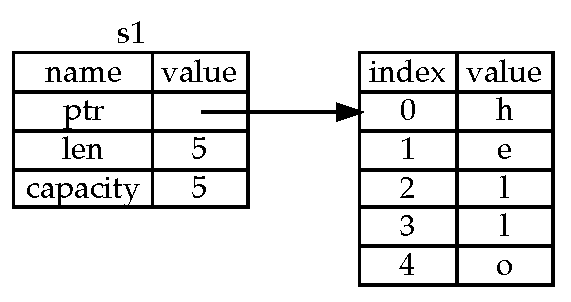
\includegraphics[scale=0.9]{Programmierung/Tabelle1.pdf}
    \caption{Repräsentation des Speichers eines String}
    \label{fig:tabelle1}
\end{figure}

\autoref{fig:tabelle1} zeigt die Bestandteile eines String. Er besteht aus drei Teilen, zu sehen in der linken Tabelle: ein Pointer auf den Speicher, der den String enthält, die Länge und die Kapazität. Wenn die Kapazität nicht mehr ausreicht, vergrößert sie sich automatisch. Dabei wird der Speicherplatz nach jeder erneuten Allokation verdoppelt. Diese Datengruppe wird auf dem Stack gespeichert. In der rechten Tabelle ist sich der Speicher auf dem Heap dargestellt.

\begin{figure}[htbp]
    \centering
    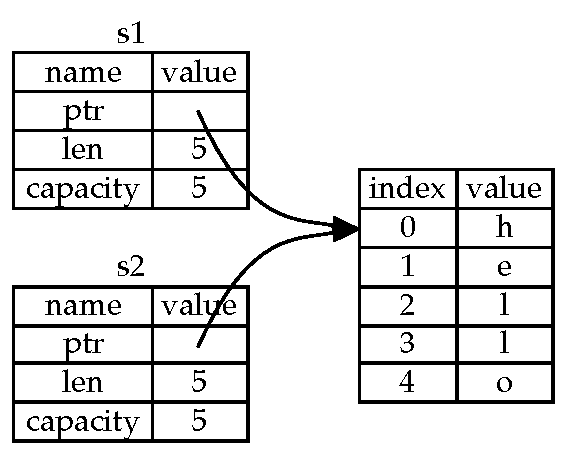
\includegraphics[scale=0.9]{Programmierung/Tabelle2.pdf}
    \caption{Repräsentation des Speichers eines String: Kopie}
    \label{fig:tabelle2}
\end{figure}

Im letzten Codebeispiel werden bei der Zuweisung von \verb"s1" zu \verb"s2" nur die Stringdaten, also ein Pointer, die Länge und die Kapazität kopiert, welche sich auf dem Stack befinden. Die Daten des Heaps werden nicht kopiert. \autoref{fig:tabelle2} zeigt eine mögliche Darstellung.

Wenn Rust eine vollständige Kopie gemacht hätte, würden die Daten wie auf \autoref{fig:tabelle3} aussehen und die Operation \verb"s2 = s1" wäre hinsichtlich der Lauf\-zeit\-leis\-tung sehr teuer.

\begin{figure}[htbp]
    \centering
    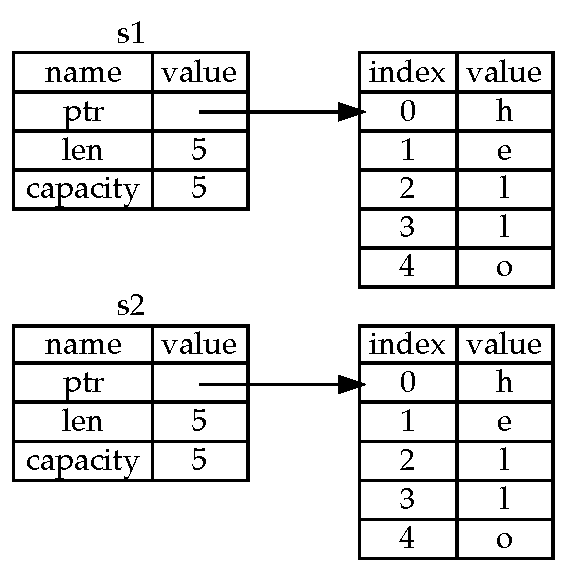
\includegraphics[scale=0.9]{Programmierung/Tabelle3.pdf}
    \caption{Repräsentation des Speichers eines String: Vollständige Kopie}
    \label{fig:tabelle3}
\end{figure}

Sobald eine Variable außerhalb des Gültigkeitsbereichs der Lebensdauer gelangt, wird der Spei\-cher aus dem Heap gelöscht. Aber da der Speicherbereich in \autoref{fig:tabelle2} von zwei Variablen referenziert wird, würde zwei mal der Speicherbereich freigegeben werden. Das ist bekannt als \glqq double free\grqq{}-Error und kann zu Speicherbeschädigungen und Sicherheitsanfälligkeiten führen.

Um die Speichersicherheit zu gewährleisten, hält Rust \verb"s1" für ungültig und muss somit nichts löschen, wenn \verb"s1" die Lebensdauer verlässt.

Das hat zur Folge, dass \verb"s1" nicht mehr genutzt werden kann, nachdem es \verb"s2" zugewiesen wurde:

\begin{lstlisting}
    let s1 = String::From("hello");
    let s2 = s1;
    println!("{}, world!", s1);         // error
\end{lstlisting}

Daraus entsteht folgende Fehlermeldung:

\begin{lstlisting}
    error[E0382]: borrow of moved value: `s1`
     --> src/main.rs:5:28
    3 |     let s1 = String::from("hello");
      |         -- move occurs because `s1` has type
    `std::string::String`, which does not implement the
    `Copy` trait
    4 |     let s2 = s1;
      |              -- value moved here
    5 |     println!("{}, world!", s1);
      |                            ^^ value borrowed here
    after move
\end{lstlisting}

Diese Art von Kopieren, welche die erste Variable ungültig macht, wird in Rust \glqq move\grqq{} genannt (\verb"s1" was \textit{moved} into \verb"s2"). Was also tatsächlich passiert, wird in \autoref{fig:tabelle4} dargestellt.

\begin{figure}[htbp]
    \centering
    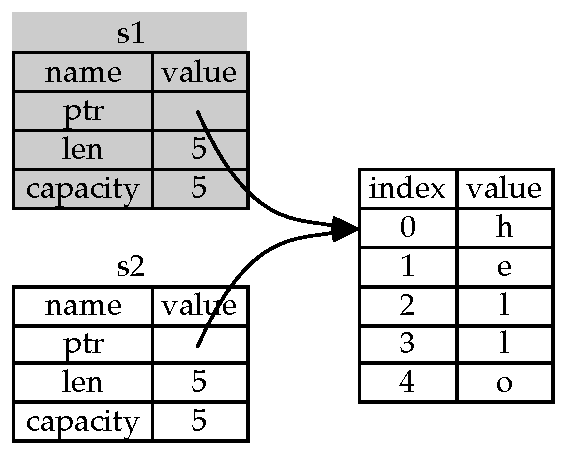
\includegraphics[scale=0.9]{Programmierung/Tabelle4.pdf}
    \caption{Repräsentation des Speichers eines String: Moved}
    \label{fig:tabelle4}
\end{figure}

Folglich gibt es in Rust keinen \glqq double free\grqq{}-Error, da der Speicher nur einmal freigegeben wird, nämlich wenn \verb"s2" den Gültigkeitsbereich verlässt.

\newpage

\subsubsection{Variablen und Daten: Clone}

Wenn eine vollständige Kopie erstellt werden soll, kann die Methode \verb"clone" benutzt werden:

\begin{lstlisting}
    let s1 = String::from("hello");
    let s2 = s1.clone();

    println!("s1 = {}, s2 = {}", s1, s2);
\end{lstlisting}

Der Code kompiliert ohne Fehlermeldungen und erzeugt explizit das in \autoref{fig:tabelle3} gezeigte Verhalten, bei dem auch die Heap-Daten kopiert werden.

\subsubsection{Ownership und Funktionen}

Die Semantik bezüglich Ownership für die Übergabe eines Wertes an eine Funktion ähnelt derjenigen, die einer Variablen einen Wert zuweist. Beim Übergeben von Variablen an eine Funktion wird genauso wie bei einer Zuweisung die Ownership übergeben (Move), wenn es sich um keinen einfachen Skalarwert handelt. Wie in C/C++ werden die Daten bei der Übergabe an Funktionen kopiert (in Rust: \autoref{fig:tabelle4}), wenn kein Pointer verwendet wird, also \glqq call by value\grqq{}. Pointer werden in Rust Referenzen genannt. Die Funktionsweise von Referenzen wird in \autoref{chap:ref} erklärt.

Folgendes Programm zeigt, wie die Ownership von Variablen übergeben werden:

\begin{lstlisting}
    fn main() {
        let s = String::from("hello");
        takes_ownership(s);

        let x = 5;
        makes_copy_because_scalar(x);

        println!("{}", s); // compiler error
        println!("{}", x); // this works!
    }

    fn takes_ownership(some_string: String) {
        println!("{}", some_string);
    }
    fn makes_copy_because_scalar(some_integer: i32) {
        println!("{}", some_integer);
    }
\end{lstlisting}

Wenn \verb"s" nach der Methode \verb"takes_ownership" genutzt wird, würde Rust einen Fehler bei der Kompilierung ausgeben. Diese statischen Checks sollen Fehler im Programm verhindern.

Funktionen können Ownership durch einen Rückgabewert auch wieder zu\-rück\-ge\-ben:

\begin{lstlisting}
    fn main() {
        let s1 = gives_ownership();
        let s2 = takes_and_gives_back(s1);
        println!("{}, world!", s1); // error
        println!("{}, world!", s2); // this works
    }

    fn gives_ownership() -> String {
        let some_string = String::from("hello");
        some_string
    }

    fn takes_and_gives_back(a_string: String) -> String {
        a_string
    }
\end{lstlisting}

\subsection{Referenzen und Borrowing}\label{chap:ref}

Referenzen können verwendet werden, um einen Zeiger zu übergeben, sodass nicht der Ganze Datentyp kopiert werden muss. Also \glqq call by reference\grqq{}.

Eine Funktion, welche die Länge eines Strings berechnet und die Ownership des verwendeten Strings wieder zurückgibt, könnte so aussehen:

\begin{lstlisting}
    fn main() {
        let s1 = String::from("hello");
        let (s2, len) = calculate_length(s1);
        println!("The length of {} is {}.", s2, len);
    }
    fn calculate_length(s: String) -> (String, usize) {
        let length = s.len();
        (s, length)
    }
\end{lstlisting}

Dies ist jedoch viel Aufwand für ein Konzept, das gebräuchlich sein sollte. Daher können in Rust Referenzen auf Variablen übergeben werden.

So wird die \verb"calculate_length" Funktion definiert und benutzt, die eine Referenz auf ein Objekt als Parameter enthält, anstatt die Ownership zu übernehmen:

\begin{lstlisting}
    fn main() {
        let s1 = String::from("hello");
        let len = calculate_length(&s1);
        println!("The length of {} is {}.", s1, len);
    }
    fn calculate_length(s: &String) -> usize {
        s.len()
    }
\end{lstlisting}

Der gesamte Tupelcode in der Variablendeklaration und der Funk\-ti\-ons\-rück\-ga\-be\-wert ist weg. Außerdem wird \verb"&s1" in \verb"calculate_length" und in seiner Definition \verb"&String" anstelle von \verb"String" benutzt.

Die \verb"&"-Zeichen erstellen Referenzen, die auf einen bestimmten Wert verweisen, ohne dessen Ownership zu beanspruchen. \autoref{fig:tabelle5} zeigt ein Diagramm.

\begin{figure}[htbp]
    \centering
    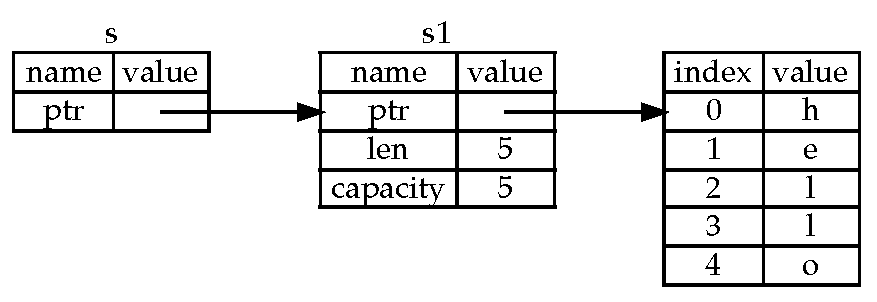
\includegraphics[scale=0.9]{Programmierung/Tabelle5.pdf}
    \caption{Diagramm von Zeiger \texttt{\&String} \texttt{s} auf \texttt{String} \texttt{s1}}
    \label{fig:tabelle5}
\end{figure}

Mit der \verb"&s1" Syntax kann eine Referenz erstellt werden, die sich auf den Wert von \verb"s1" bezieht, ihm aber nicht gehört. Der Wert auf den er verweist wird nicht gelöscht, wenn die Referenz den Gültigkeitsbereich verlässt.

Ebenso verwendet die Signatur der Funktion \verb"&" um anzuzeigen, dass der Typ des Parameters eine Referenz ist.

Das Gegenteil der Referenzierung mit \verb"&" ist die Dereferenzierung, die mit dem Dereferenzierungsoperator \verb"*" erzielt wird.

Die Lebensdauer von Referenzen, ist die, eines normalen Funktionsparameters, jedoch wird der Wert nicht aus dem Speicher gelöscht, da keine Ownership übergeben wurde. Referenzierung im Funktionsparameter wird in Rust \glqq borrowing\grqq{} genannt. Wie in der realen Welt kann Eigentum an andere ausgeliehen werden. Wenn die andere Person es nicht mehr braucht, kann diese es wieder an den Eigentümer zurückgeben.

Genauso wie Variablen standardmäßig unveränderlich sind, gilt dies auch für Referenzen. Es kann nichts verändert werden, auf das nur mit \verb"&" referenziert wird. Folgender Code würde daher nicht funktionieren:

\begin{lstlisting}
    fn main() {
        let s = String::from("hello");
        change(&s);
    }
    fn change(some_string: &String) {
        some_string.push_str(", world"); // compiler error
    }
\end{lstlisting}

\subsubsection{Veränderbare Referenzen}

Kleine Veränderungen beheben den Fehler aus dem letzten Codebeispiel:

\begin{lstlisting}
    fn main() {
        let mut s = String::from("hello");
        change(&mut s);
    }
    fn change(some_string: &mut String) {
        some_string.push_str(", world"); // works now
    }
\end{lstlisting}

Die Variable \verb"s" muss durch Kennzeichnung mit \verb"mut" veränderbar gemacht werden. Außerdem wird nun eine veränderbare Referenz übergeben (\verb"&mut"). Die Funktion erwartet nun eine entsprechende Referenz als Parameter in der Form: \verb"some_string:" \verb"&mut String".

Es gibt jedoch eine große Einschränkung: Es darf nur eine veränderbare Referenz auf ein bestimmtes Datenelement in einem bestimmeten Bereich aktiv sein. Folgender Code würde somit nicht kompilieren:

\begin{lstlisting}
    let mut s = String::from("hello");
    let r1 = &mut s;
    let r2 = &mut s;                    // error
    println!("{}, {}", r1, r2);
\end{lstlisting}

Diese Einschränkung erlaubt kontrollierte Verwendung von Variablen. Mithilfe dieser Regel verhindert Rust sogenannte \glqq data races\grqq{}. Diese ähneln \glqq race conditions\grqq{} und treten auf, wenn drei Verhaltensweisen auftreten:

\begin{itemize}
    \item Zwei oder mehr Pointer greifen zeitgleich auf den selben Speicherbereich zu.
    \item Mindestens einer der Pointer schreibt.
    \item Kein Mechanismus wird verwendet, um den Zugriff der Daten zu synchronisieren.
\end{itemize}

Diese \glqq data races\grqq{} können undefiniertes Verhalten auslösen und sind schwer festzustellen und zu beheben. In Rust-Programmen gibt es dieses Problem nicht, da gefährdeter Code nicht fehlerfrei kompilieren kann.

Es dürfen auch keine Kombinationen aus veränderbaren und unveränderbaren Referenzen erstellt werden. Folgender Code führt zu einem Compilerfehler:

\begin{lstlisting}
    let mut s = String::from("hello");
    let r1 = &s;     // ok
    let r2 = &s;     // ok
    let r3 = &mut s; // error
\end{lstlisting}

Bei unveränderlichen Referenzen sollten man nicht damit rechnen müssen, dass sich der Wert dahinter verändern kann. Mehrere unveränderbare Referenzen sind in Ordnung, da mehrere lesende Zugriffe sich untereinander nicht beeinflussen.

\subsubsection{\glqq Dangling References\grqq{}}

In Programmiersprachen mit Pointern kann es vorkommen, dass diese auf einen Bereich im Speicher zeigen, der bereits freigegeben wurde. Das sind sogenannte \glqq dangling pointer\grqq{}. In Rust garantiert der Compiler, dass Referenzen immer auf einen gültigen Bereich zeigen. Folgender Code wird also beim Kompilieren eine Fehlermeldung ausgeben:

\begin{lstlisting}
    fn main() {
        let reference_to_nothing = dangle();
    }
    fn dangle() -> &String {
        let s = String::from("hello");
        &s
    }
\end{lstlisting}

Der String \verb"s" wird nach der Funktion \verb"dangle" aus dem Speicher gelöscht. Die Referenz, die zurückgegeben wird, zeigt auf einen ungültigen Bereich im Speicher. Der Compiler erkennt, dass der Rückgabewert eine \glqq dangling reference\grqq{} ist und gibt eine Fehlermeldung aus. Damit der String im Speicher bleibt, muss die Ownership von \verb"s" zurückgegeben werden:

\begin{lstlisting}
    fn no_dangle() -> String {
        let s = String::from("hello");
        s
    }
\end{lstlisting}

\subsubsection{Regeln: Referenzen}

\begin{itemize}
    \item Es kann entweder nur eine veränderbare oder eine beliebige Anzahl an unveränderlichen Referenzen gleichzeitig benutzt werden.
    \item Referenzen müssen immer auf einen gültigen Bereich zeigen.
\end{itemize}

\subsection{Slice Typ}\label{chap:slice}

Ein weiterer Datentyp, welcher keine Ownership annimmt sind Slices. Sie werden benutzt um eine zusammenhängende Folge von Elementen einer Sammlung anstatt auf die gesamte Sammlung zu verweisen.

\subsubsection{String Slice}

In Rust kann mit sogenannten \glqq string slices\grqq{} ein bestimmter Bereich eines Strings referenziert werden.

\begin{lstlisting}
    let s = String::from("hello world");
    let hello = &s[0..5];
    let world = &s[6..11];
\end{lstlisting}

Die Syntax der Klammern beschreibt \verb"[starting_index..ending_index]". Intern wird die Startposition und die Länge gespeichert. Die Länge errechnet sich aus der Differenz von \verb"starting_index" und \verb"ending_index". \verb"world" ist ein Pointer auf das siebte Byte von \verb"s" mit einer Länge von 5. \autoref{fig:tabelle6} zeigt ein Diagramm des Speichers.

\begin{figure}[htbp]
    \centering
    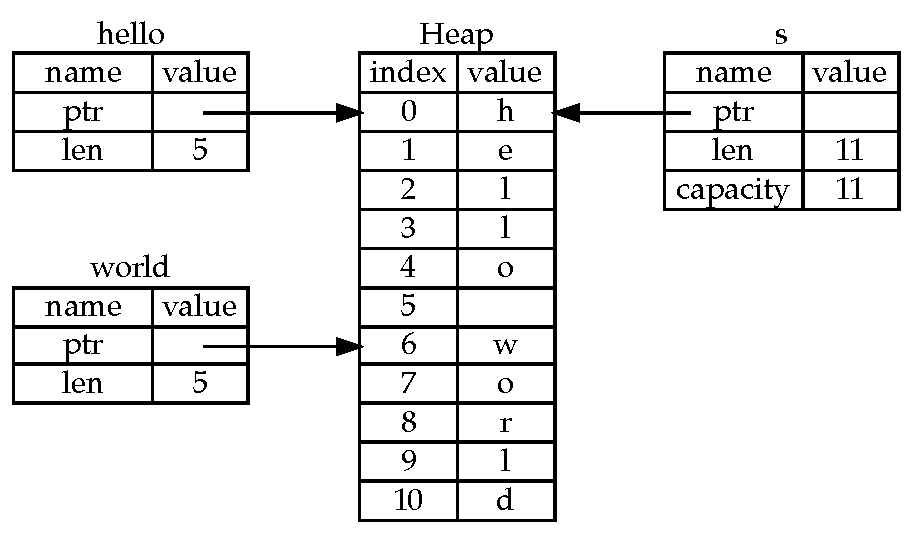
\includegraphics[scale=0.9]{Programmierung/Tabelle6.pdf}
    \caption{Diagramm von String Slices}
    \label{fig:tabelle6}
\end{figure}

Dadurch entsteht eine Abhängigkeit, welche es Rust erlaubt, bereits beim Kompilieren festzustellen, ob String Slices auf einen gültigen Bereich im Speicher zeigen. So wird der Code weniger anfällig für Laufzeitfehler.

\begin{lstlisting}
    let s = "Hello, world!";
\end{lstlisting}

Der Typ von \verb"s" ist \verb"&str": Es ist ein String Slice, der auf einen bestimmten Bereich einer Zeichenkette verweist. Deshalb sind String Literale unveränderlich. \verb"&str" ist eine unveränderliche Referenz.

\subsubsection{Andere Slices}

String Slices sind speziell für Strings. Es gibt auch einen allgemeineren Slice Typ für Felder, bei dem wie bei String Slices auch hier Teile von Felder referenziert werden können:

\begin{lstlisting}
    let a = [1, 2, 3, 4, 5];
    let slice = &a[1..3];
\end{lstlisting}

Der Typ von \verb"slice" ist \verb"&[i32]". Auch hier wird ein Pointer auf das erste Element sowie die Länge des Slice gespeichert.

Wie in \autoref{chap:array} erwähnt, können Slices dazu verwendet werden, Felder an Funktionen über einen \glqq call by reference\grqq{} zu übergeben:

\begin{lstlisting}
    fn main() {
        let array = [1, 2, 3, 4, 5];
        call_by_reference(&array);
    }
    
    fn call_by_reference(slice: &[i32]) {
        for element in slice.iter() {
            println!("{}", element);
        }
    }
\end{lstlisting}

\subsection{Lifetime Operator}

Folgende Funktion gibt eine Referenz eines Inputs zurück:

\begin{lstlisting}
    fn ref_test(a: &i32, b: &i32) -> &i32 {
        a
    }
\end{lstlisting}

Bei Aufruf dieser Funktion entsteht ein Problem:

\begin{lstlisting}
    fn main() {
        let a = 549;

        let e;
        {
            let tmp = a;
            e = ref_test(&a, &tmp); // e is a reference of a
        }
        // tmp goes out of scope

        // cant use e because tmp does not live long enough
        println!("{}", e);
    }
\end{lstlisting}

Der Compiler kann nicht feststellen, ob die Lebensdauer des Rückgabewerts von der Lebensdauer der übergebenen Referenzen abhängig ist. Darum müssen die Lebenszeiten mit dem Lifetime Operator im Funktionskopf angegeben werden.

\begin{lstlisting}
    // doesn't work yet
    fn ref_test<'a>(a: &'a i32, b: &'a i32) -> &'a i32 {
        a
    }
\end{lstlisting}

Lifetimes werden in Rust mit einem Apostroph geschrieben. Obiger Code de\-fi\-niert eine Lebensdauer \verb"'a" in den spitzen Klammern. Den Parametern und dem Rückgabewert wird diese Lebensdauer zugeordnet. Der Compiler interpretiert daraus, dass beide Parameter die gleiche Lebensdauer haben könnten. Damit der Code aus der \verb"main" Funktion fehlerfrei kompiliert werden kann, muss der Parameter \verb"b" mit einer anderen Lebensdauer markiert werden:

\begin{lstlisting}
    // now it works
    fn ref_test<'a, 'b>(a: &'a i32, b: &'b i32) -> &'a i32 {
        a
    }
\end{lstlisting}

Jetzt weiß der Compiler, dass die Lebendauer des Rückgabewerts abhängig vom ersten Parameter \verb"a" ist. Es kann also sichergestellt werden, dass der Wert hinter der Referenz \verb"e" nach dem Block weiterlebt.

\section{Modulsystem}

Dieses System von Rust ermöglicht die Erstellung von Modulen, welche mit Pfaden angesprochen werden können. Hiermit können auch externe Pakete verwendet werden:

Module lassen den Code in Gruppen einteilen:

\begin{lstlisting}
    mod sound {
        mod instrument {
            mod string {
                fn guitar() {}
            }
        }
        mod voice {}
    }
\end{lstlisting}

Das Beispiel definiert das Modul \verb"sound" mit zwei inneren Modulen \verb"instrument" und \verb"voice" und ein Modul \verb"string" in \verb"instrument" mit der Funktion \verb"guitar". Der gesamte Modulbaum ist unter dem impliziten Modul namens \verb"crate" verwurzelt.

Diese Art von Baum erinnert an das Dateisystem eines Betriebssystems. Genau wie Verzeichnisse in einem Dateisystem, kann im Code durch Module Code or\-ga\-ni\-siert werden. Eine weitere Ähnlichkeit zu Dateisystemen besteht darin, dass zum Verweisen auf ein Element dessen Pfad verwendet wird.

Es gibt zwei Arten von Pfaden:

\begin{itemize}
    \item Ein absoluter Pfad beginnend beim crate root mithilfe des crate-Namens oder dem Schlüsselwort \verb"crate".
    \item Ein relativer Pfad beginnend beim aktuellen Modul, er verwendet \verb"self", \verb"super" oder einen Bezeichner im aktuellen Modul.
\end{itemize}

Das Trennzeichen besteht aus zwei Doppelpunkten (\verb"::"). Folgende \verb"main"-Funktion könnte unter dem letzten Codebeispiel folgen:

\begin{lstlisting}
    fn main() {
        // absolute path
        crate::sound::instrument::string::guitar();

        // relative path
        sound::instrument::string::guitar();
    }
\end{lstlisting}

Dieser Code würde jedoch nicht kompilieren, da alle Elemente (Funktionen, Methoden, Strukturen, Enums und Konstanten) standardmäßig privat sind. Um ein Element öffentlich zu machen, kann das Schlüsselwort \verb"pub" verwendet werden.

Elemente ohne das Schlüsselwort \verb"pub" sind privat, wenn der Modulbaum des aktuellen Moduls \glqq nach unten\grqq{} betrachtet wird. Elemente ohne \verb"pub" sind jedoch öffentlich, wenn sich diese auf derselben Ebene befinden, oder der Baum \glqq nach oben\grqq{} betrachtet wird. In einem Dateisystem verhält es sich ähnlich: Ohne Berechtigung auf einen Ordner kann dieser nicht betrachtet werden. Auf einen zugänglichen Ordner können dessen Vorgängerverzeichnisse auch eingesehen werden.

Um die Funktion \verb"guitar" in der \verb"main"-Methode aufrufen zu können, müssen ei\-ni\-ge Module sowie die Funktion öffentlich gemacht werden:

\newpage

\begin{lstlisting}
    mod sound {
        pub mod instrument {
            pub mod string {
                pub fn guitar() {}
            }
        }
        mod voice {}
    }
\end{lstlisting}

Relative Pfade können mit \verb"super" auch auf übergeordnete Module zugreifen, ähnlich wie bei einem Dateisystem mit \glqq\verb".."\grqq{}:

\begin{lstlisting}
    mod sound {
        pub mod instrument {
            pub fn clarinet() {
                super::breathe_in();
            }
        }
        fn breathe_in() {
            // Function body code
        }
    }
\end{lstlisting}

Häufig genutzte Pfade können mit dem Schlüsselwort \verb"use" gekürzt werden. Das ist vergleichbar mit einer Verknüpfung in einem Dateisystem. Es können absolute und relative Pfade benutzt werden.

\begin{lstlisting}
    use crate::sound::instrument;

    fn main() {
        instrument::clarinet();
    }
\end{lstlisting}

Externe Pakete können mit \verb"use"  eingebunden werden. Dafür muss zunächst das Paket via Cargo.toml hinzugefügt werden:

\begin{lstlisting}
    [dependencies]
    rand = "0.6.5"
\end{lstlisting}

\newpage

\noindent Im Code würde das so aussehen:

\begin{lstlisting}
    use rand::Rng;

    fn main() {
        let secret = rand::thread_rng().gen_range(1, 101);
    }
\end{lstlisting}

Der Quellcode kann mit dem Schlüsselwort \verb"mod" auf mehrere Dateien aufgeteilt werden. Dabei ist der Name der Datei der Name des Moduls. Ordnerstrukturen können auch erstellt werden. Dabei ist der Ordner selbst auch ein Modul, dessen Definition in der Datei \verb"mod.rs" definiert werden kann.

\vspace{0.5cm}

\noindent Datei \textbf{src/main.rs}

\begin{lstlisting}
    mod sound;

    fn main() {
        sound::instrument::clarinet();
    }
\end{lstlisting}

\vspace{0.5cm}

\noindent Datei \textbf{src/sound.rs}

\begin{lstlisting}
    pub mod instrument {
        pub fn clarinet() {
            // Function body
        }
    }
\end{lstlisting}


\section{Objektorientierung}\label{chap:oop}

In der Programmiergemeinschaft herrscht kein Konsens darüber, welche Merkmale eine Sprache besitzen muss, um objektorientiert zu sein. Rust wird von vielen Programmierparadigmen beeinflusst, darunter auch von objektorientierter Programmierung (OOP). Objektorientierte Sprachen teilen üblicherweise drei Gemeinsamkeiten: Objekte, Kapselung und Vererbung.

Das Buch \textit{Design Patterns: Elements of Reusable Object-Oriented Software} von Erich Gamma, Richard Helm, Ralph Johnson und John Vlissides definiert OOP auf diese Weise:

\begin{quote}
    Object-oriented programs are made up of objects. An object packages both data and the procedures that operate on that data. The procedures are typically called methods or operations.
\end{quote}

Nach dieser Definition ist Rust objektorientiert. Strukturen und Enums enthalten Daten, \verb"impl" Blöcke stellen Methoden für diese bereit.

Eine Struktur in Rust ist vergleichbar mit \verb"struct" in C. Rust kann diese Strukturen jedoch mit Methoden erweitern, sodass diese wie Klassen verwendet werden können. So wird eine Struktur mit drei Deklarationen \verb"id", \verb"age" und \verb"wage" definiert:

\begin{lstlisting}
    struct Employee {
        id: i32,
        age: i32,
        wage: f64,
    }
    
    impl Employee {
        fn new(id: i32, age: i32, wage: f64) -> Self {
            Employee { id, age, wage }
        }
        fn birthday(&mut self) {
            self.age += 1;
        }
    }
    
    fn main() {
        let mut joe = Employee::new(1, 32, 48000.0);
        joe.birthday();
    }
\end{lstlisting}

Die Methode \verb"new" ist der Konstruktor, dessen Rückgabetyp \verb"Self" ist. \verb"Self" ist der Typ von \verb"impl". Er könnte auch mit \verb"-> Employee" definiert sein. Alternativ kann eine Instanz auch ohne Konstruktor erstellt werden:

\begin{lstlisting}
    let mut joe = Employee {
        id: 1,
        age: 32,
        wage: 48000.0,
    };
\end{lstlisting}

Wenn in Methoden auf das eigene Objekt zugegriffen werden soll, muss dieses als ersten Funktionsparameter übergeben werden. Diese Übergabe geschieht automatisch: beim Aufruf \verb"joe.birthday();" muss innerhalb der Klammern nichts geschrieben werden.

\subsection{Stack oder Heap?}

In C++ werden Objekte auf dem Stack gespeichert, wenn kein \verb"new" Operator verwendet wird. In Rust werden Objekte zunächst auch auf dem Stack gespeichert.

C++ Code:

\begin{lstlisting}
    Employee e(1, 32, 48000.0);
\end{lstlisting}

Rust Code:

\begin{lstlisting}
    let e = Employee::new(1, 32, 48000.0);
\end{lstlisting}

Soll in C++ ein Objekt auf dem Heap alloziert werden, wird der \verb"new" Operator verwendet. In Rust muss ein sogenannter Smart Pointer erstellt werden. Die Funktionsweise von Smart Pointer wird in \autoref{chap:smpointer} erläutert. Zunächst ist wichtig zu verstehen, dass in Rust jeder Datentyp auf dem Heap gespeichert werden kann.

C++ Code:

\begin{lstlisting}
    Employee *e = new Employee(1, 32, 48000.0);
    delete e;
\end{lstlisting}

Rust Code:

\begin{lstlisting}
    let e = Box::new(Employee::new(1, 32, 48000.0));
\end{lstlisting}

\subsection{Smart Pointer}\label{chap:smpointer}

Smart Pointer in Rust verhalten sich ähnlich wie Referenzen, mit dem Unterschied, dass sie mit einem Konstruktoraufruf instanziiert werden können. Sie sind also Strukturen bzw Klassen, die einen Pointer auf einen beliebigen Typ beinhalten. Genau wie Referenzen können sie mit dem \verb"*" Operator dereferenziert werden. Es gibt verschiedene Smart Pointer, häufig genutzt werden folgende drei Arten:

\begin{itemize}
    \item \verb"Box<T>" wird verwendet, um Werte dem Stack zuzuweisen.
    \item \verb"Rc<T>" erlaubt das Teilen von Ownership, realisert wird das durch Zählen von Referenzen.
    \item \verb"Arc<T>" erlaubt das Teilen von Ownership für mehrere Threads, wenn ein Synchronisierungsmechanismus benutzt wird.
\end{itemize}

\subsubsection{Verwendung von \texttt{Box<T>}}

Der \verb"Box<T>" Typ kann auch dazu verwendet werden, Ownership von großen Datentypen zu übertragen. So kann das Kopieren von vielen Daten ausgeschlossen werden.

\begin{lstlisting}
    fn main() {
        let large = Box::new(LargeStruct::new());
        take_boxed_ownership(large);
        // large is now invalid
    }
    
    fn take_boxed_ownership(x: Box<LargeStruct>) {
        // do stuff
    }
\end{lstlisting}

\subsection{Kapselung}

Ein weiterer Aspekt, welcher häufig mit OOP in Verbindung steht, ist die Idee der Kapselung. Das bedeutet, dass die Implementierung eines Objekts nicht für den Code verfügbar ist, der dieses Objekt verwendet.

Mit Modulen kann in Rust gekapselt werden. Aber auch Strukturen und Enums, sowie dessen Werte, sind standardmäßig privat und können mit dem Schlüsselwort \verb"pub" öffentlich gemacht werden.

\begin{lstlisting}
    pub mod people {
        pub struct Employee {
            pub id: i32,  // public
            age: i32,     // private
            wage: f64,    // private
        }
    }
\end{lstlisting}

\subsection{Vererbung}

Vererbung ist ein Mechanismus, mit dem ein Objekt von der Definition eines anderen Objekts erben kann, wodurch die Daten und das Verhalten des über\-ge\-ord\-ne\-ten Objekts übernommen werden, ohne dass sie erneut definiert werden müssen.

Wenn eine Sprache Vererbung können muss, um eine objektorientierte Sprache zu sein, dann ist Rust keine. Es gibt keine Möglichkeit eine Struktur zu definieren, die Felder und Methodenimplementierungen der übergeordneten Struktur erbt.

Ein Beispiel der Vererbung in C++:

\begin{lstlisting}
    class Employee {
      public:
        string first_name, family_name;
        char middle_initial;
        Date hiring_date;
        short department;
        // ...
    };

    class Manager : public Employee {
        list<Employee *> group;
        short level;
        // ...
    };
\end{lstlisting}

Hier besitzt der Manager die gleichen Felder wie ein normaler Mitarbeiter, zu\-sätz\-lich zu den eigenen Feldern.

\subsubsection{Warum verzichtet Rust auf Vererbung?}

In letzter Zeit ist die Vererbung als Entwurfslösung in vielen Programmiersprachen in Ungnade gefallen, da häufig die Gefahr besteht, dass mehr Code als erforderlich gemeinsam genutzt wird. Unterklassen sollten nicht immer alle Merkmale ihrer übergeordneten Klasse gemeinsam haben, dies geschieht jedoch mit Vererbung. Das kann das Design eines Programms weniger flexibel machen. Außerdem wird die Möglichkeit eingeführt, Methoden für Unterklassen aufzurufen, die keinen Sinn ergeben, oder Fehler verursachen, da die Methoden nicht für die Unterklasse gelten. Darüber hinaus können in einigen Sprachen nur Unterklassen von einer Klasse erben, wodurch die Flexibilität der Sprache weiter einschränkt wird.

\subsection{Traits}

Ein \verb"trait" ist eine Sammlung von Methoden, die für einen unbekannten Typ definiert werden: \verb"Self". Sie können auf Methoden zugreifen, die im selben Trait definiert sind. Traits können für jeden Datentyp implementiert werden. \cite{RustExample}

\begin{lstlisting}
    pub trait Animal {
        fn noise(&self) -> &str;
    }
\end{lstlisting}

Dieses Trait definiert ein Tier, welches Geräusche von sich geben kann.

\begin{lstlisting}
    pub struct Sheep {
        pub name: String,
    }
    impl Animal for Sheep {
        fn noise(&self) -> &str {
            "baaaaaah"
        }
    }
\end{lstlisting}

Die Struktur \verb"Sheep" implementiert den Trait, sodass ein Schaf als Tier gesehen wird. Es kann nun eine Funktionen geschrieben werden, die ein beliebiges Tier erwartet:

\begin{lstlisting}
    pub fn make_animal_speak(animal: &dyn Animal) {
        println!("Animal says {}.", animal.noise());
    }
\end{lstlisting}

Es können auch Vektoren mit Trait-Objekten erstellt werden:

\begin{lstlisting}
    let mut animals: Vec<Box<dyn Animal>> = Vec::new();
    animals.push(Box::new(Sheep {}));
\end{lstlisting}

Das Schlüsselwort \verb"dyn" ist optional, dient aber zur besseren Unterscheidung zwi\-schen einem Trait (dyn) und einer Struktur und sollte daher bei Traitobjekten immer verwendet werden. Da \verb"Animal" nur ein Trait ist und keine Struktur, wird das Schlüsselwort benutzt.

% TODO Box
Der Typ \verb"Box" ist ein Pointer mit einer festen Speichergröße, mit dem Werte auf dem Heap gespeichert werden können. Er wird benötigt, da zur Kompilierzeit die Größe des Datentyps noch nicht bekannt ist.

\subsubsection{Trait-Objekte benutzen dynamische Bindung (dynamic dispatch)}\label{dynamicdispatch}

Wenn Trait-Objekte für Funktionen verwendet werden, muss Rust die dynamische Bindung benutzen. Der Compiler kennt nicht alle Typen, die möglicherweise für den Code verwendet werden. Er weiß also nicht, welche Methode für welchen Typ der Aufruf implementiert ist. Daher verwendet Rust zur Laufzeit Zeiger im Trait-Objekt, um zu ermitteln, welche Methode aufgerufen werden soll. Wenn diese Suche ausgeführt wird, fallen Laufzeitkosten an, die beim statischen Binden (sta\-tic dispatch) nicht auftreten würden. Die dynamische Bindung verhindert auch, dass der Compiler den Code einer Methode direkt an die entsprechende Stelle kopiert, wodurch Optimierungen verhindert werden können. Jedoch erhält man durch Traits zusätzliche Flexibilität im Code. Es ist also ein Kompromiss.

\section{Generische Programmierung}

Ähnlich wie in C++ (Templates) gibt es auch in Rust die Möglichkeit, Typen als Argumente zu übergeben, ohne Informationen zu verlieren. Das bedeutet: Es können Funktionssignaturen oder Strukturen erstellt werden für Elemente, die viele verschiedene konkrete Datentypen verwenden können.

Beispiel in Rust:

\begin{lstlisting}
    struct Point<T> {
        x: T,
        y: T,
    }
    
    impl<T> Point<T> {
        fn new(x: T, y: T) -> Point<T> {
            Point { x: x, y: y }
        }
    }
    
    fn main() {
        let p1 = Point::new(1, 2);
        let p2 = Point::new(1.0, 2.0);
    }
\end{lstlisting}

Die Klasse \verb"Point" beinhaltet zwei Werte, deren Typen erst bei der Erstellung des Objekts bekannt werden. Beide Variablen \verb"x" und \verb"y" haben den gleichen Typ \verb"T". Die Variable \verb"p1" ist ein \verb"Point<i32>" und \verb"p2" ein \verb"Point<f64>".

Es können auch Typen verwendet werden, die bestimmte Traits implementieren müssen:

\begin{lstlisting}
    fn animal_noise<T: Animal>(animal: T) {
        println!("This animal makes {}.", animal.noise());
    }
\end{lstlisting}

C++ und Rust implementieren Generics so, dass Code mit generischen Typen nicht langsamer läuft als mit konkreten Typen. Rust erreicht dies dadurch, dass beim Kompilieren generischer Code in spezifischen Code umgewandelt wird und die konkreten Typen eingetragen werden. Dieser Prozess wird Monomorphisierung genannt.


\section{Unit-Tests}\label{chap:unittests}
Bei der Entwicklung von Rust wurde auf ein möglichst hohes Maß an Fehlerfreiheit in Programmen geachtet. Fehlerfreiheit ist jedoch nur schwer nachzuweisen. Das Typensystem von Rust kann nicht jede Art von Fehler verhindern, daher bietet Rust Unterstützung für das Schreiben automatisierter Softwaretests.

In C oder C++ gibt es Frameworks, welche von Dritten angeboten werden. Ein Beispiel ist Google Test\footnote{https://github.com/google/googletest}.

Für Unit-Tests in Rust wird nach Konvention in jeder Datei ein Modul mit dem Namen \verb"tests" erstellt mit der Annotation \verb"#[cfg(test)]". Hier werden Testfunktionen definiert mit der Annotation \verb"#[test]". Der Test \verb"it_works" wird mit dem Befehl \verb"cargo test" gestartet.

\begin{lstlisting}
    #[cfg(test)]
    mod tests {
        #[test]
        fn it_works() {
            assert_eq!(2 + 2, 4);       // assert equal
            assert_ne!(2 + 2, 22);      // assert not equal
        }
    }
\end{lstlisting}

Folgende Makros sind hilfreich bei der Erstellung von Tests:

\begin{itemize}
    \item \verb"assert!(a)": Prüft einen booleschen Ausdruck; Panik bei \verb"false".
    \item \verb"assert_eq!(a,b)": Vergleicht zwei Werte; Panik bei unterschiedlichen Werten.
    \item \verb"assert_ne!(a,b)": Wie \verb"assert_eq!"; Panik bei gleichen Werten.
    \item \verb"panic!()": Generiert Panik und der Test schlägt fehl.
\end{itemize}

Diese Makros können zusätzlich einen Text für mehr Informationen ausgeben:

\begin{lstlisting}
    assert_eq!(a, b, "Testing equality of {} and {}", a, b);
\end{lstlisting}


\section{Error Handling}

\subsection{Fehler mit \texttt{panic!}}

Wenn im Code ein Fehler auftritt, kann das Makro \verb"panic!" benutzt werden. In \autoref{chap:unittests} wurde es bereits benutzt, um Tests fehlschlagen zu lassen. Beim Aufruf dieses Makros gibt das Programm eine Fehlermeldung aus, räumt Stack und Heap auf und beendet sich. Paniken werden immer zur Laufzeit ausgelöst.

Wenn also eine Panik auftritt, wird das Programm standardmäßig beendet. Das bedeutet, dass das Programm selbst noch den Speicher der Objekte wieder freigibt. Das Zurückgehen des Stacks und das Aufräumen, ist jedoch eine Menge Arbeit. Die Alternative ist, sofort abzubrechen, wodurch das Programm ohne Be\-rei\-ni\-gung beendet wird und der vom Programm verwendete Speicher vom Be\-triebs\-sys\-tem bereinigt werden muss. Wenn in einem Projekt die resultierende Binärdatei so klein wie möglich gestaltet werden soll, kann bei einer Panik vom \glqq Abwickeln\grqq{} auf \glqq Abbrechen\grqq{} gewechselt werden, indem in der Cargo.toml \verb"panic = 'abort'" in die entsprechenden Abschnitte geschrieben wird:

\begin{lstlisting}
    [profile.release]
    panic = 'abort'
\end{lstlisting}

Eine Panik kann beispielsweise auch ausgelöst werden, wenn im Code auf ein Element eines Vektors zugegriffen wird, welches nicht innerhalb des Bereichs liegt:

\begin{lstlisting}
    fn main() {
        let v = vec![1, 2, 3];
        v[99];
    }
\end{lstlisting}

In diesem Codebeispiel wird mithilfe eines Makros ein Vektor mit drei Zahlen erstellt. Es wird dann auf das 99. Element zugegriffen. Dadurch entsteht folgende Fehlermeldung zur Laufzeit:

\begin{lstlisting}
    thread 'main' panicked at 'index out of bounds: the len
    is 3 but the index is 99'
\end{lstlisting}

In C und C++ würden bei Felder keine Fehlermeldungen erscheinen und es würde ein Zahlenwert ausgegeben werden, der davon abhängig ist, was in diesem Moment im Speicher steht. In C++ können alternativ Listen erstellt werden (z. B. \verb"vector<int>"), die zur Laufzeit überprüfen können, ob die Zugriffe innerhalb des Bereichs der Liste stattfinden.

\subsection{Fehler mit \texttt{Result}}

Viele Fehler sind nicht schwerwiegend genug, um ein vollständiges Anhalten des Programms zu erfordern. Wenn beispielsweise eine nicht existierende Datei geöffnet werden soll, könnte diese erstellt werden, anstatt das Programm zu beenden.

Das Enum \verb"Result" ist in der Standardbibliothek definiert:

\begin{lstlisting}
    enum Result<T, E> {
        Ok(T),
        Err(E),
    }
\end{lstlisting}

Bei \verb"T" und \verb"E" handelt es sich um generische Typparameter. Dabei stellt \verb"T" den Typ des Werts dar, der in einem Erfolgsfall innerhalb der \verb"Ok" Variante zurückgegeben wird und \verb"E" die Art des Fehlers, der in einem Fehlerfall innerhalb der \verb"Err" Variante zurückgegeben wird.

So wird eine Funktion aufgerufen, die ein \verb"Result" zurückgibt, weil sie fehlschlagen könnte.

\begin{lstlisting}
    use std::fs::File;
    fn main() {
        let f = File::open("hello.txt");
    }
\end{lstlisting}

In der Standardbibliothek steht beschrieben, welchen Typ die Funktion zu\-rück\-gibt. \verb"f" ist vom Typ \verb"Result<File, Error>". Mithilfe des \verb"match"-Statements kann getestet werden, ob die Funktion korrekt ausgeführt wurde, oder, bei Misserfolg, welche Art von Fehler entstanden ist.

\begin{lstlisting}
    use std::fs::File;
    use std::io::ErrorKind;

    let f = match f {
        Ok(file) => file,
        Err(error) => match error.kind() {
            ErrorKind::NotFound => {
                panic!() /* do stuff */
            },
            _ => panic!("could not open file"),
        },
    };
\end{lstlisting}

Der Aufruf \verb"error.kind()" gibt ein Enum \verb"ErrorKind" zurück, womit auf verschiedene Fehlerszenarien reagiert werden kann.

\subsubsection{Fehler weitergeben}

Beim Schreiben einer Funktion, welche möglicherweise einen Fehler aufruft, kann dieser an den aufrufenden Code zurückgegeben werden, anstatt ihn in dieser Funktion zu behandeln. Somit wird dem aufrufendem Code mehr Kontrolle gegeben. Anstelle des Aufrufs von \verb"panic!", wird ein \verb"return"-Statement verwendet. Alternativ kann der \verb"?"-Operator verwendet werden.

\subsection{\texttt{?}-Operator}

Wird ein \verb"?" hinter ein \verb"Result" geschrieben und der Wert ist ein \verb"Ok", wird der Wert innerhalb des \verb"Ok" von diesem Ausdruck zurückgegeben und die Funktion wird fortgesetzt. Wenn es sich bei dem Wert um einen Fehler handelt, wird der Fehler von der gesamten Funktion zurückgegeben, als ob das Schlüsselwort \verb"return" verwendet worden wäre. Dieser Operator kann nur innerhalb von Funktionen verwendet werden, welche ein \verb"Result" als Rückgabetyp haben. Dadurch wird die Implementierung vereinfacht und die Lesbarkeit des Codes verbessert.

\newpage

Codebeispiel:

\begin{lstlisting}
    use std::io;
    use std::Read;
    use std::fs::File;

    fn read_username() -> Result<String, io::Error> {
        let mut f = File::open("hello.txt")?;
        let mut s = String::new();
        f.read_to_string(&mut s)?;
        Ok(s)
    }
\end{lstlisting}

Die Methode \verb"File::open" gibt ein \verb"Result<File, io::Error>" zurück. In Ver\-bin\-dung mit dem \verb"?"-Operator wird bei erfolgreichem öffnen der Datei die Variable \verb"f" mit  dem Typ \verb"File" gesetzt. Ansonsten wird die Funktion beendet und gibt den \verb"io::Error" in einem \verb"Err" verpackt zurück. Also \verb"Err(io::Error)".

\subsection{Error Handling in C und C++}

In C gibt es keine direkte Unterstützung für die Fehlerbehandlung. Es gibt aber Möglichkeiten, wie sie dennoch durchgeführt werden kann. Viele C-Funk\-ti\-ons\-auf\-ru\-fe geben im Fehlerfall \verb"-1" oder \verb"NULL" zurück, sodass mit einer \verb"if"-Anweisung entsprechend reagiert werden kann. Die globale Variable \verb"errno" kann zusätzlich zur Unterscheidung verwendet werden.

C++ bietet einige hilfreiche Features. Die \verb"throw"-Anweisung kann Ausnahmen an einen Handler übergeben, ähnlich wie es beispielsweise in Java üblich ist. Zusätzlich können statische Assertionen benutzt werden, um zur Kompilierzeit bestimmte Eigenschaften sicherzustellen.


\section{Dokumentieren mit rustdoc}

Ein wichtiger Bestandteil bei der Programmierung in Rust ist das Erstellen von Dokumentationen. Das Tool \verb"rustdoc" ist vergleichbar mit \verb"javadoc" für Java. Es können im Code spezielle Kommentare geschrieben  und daraus eine Dokumentation mit HTML, CSS und JavaScript erstellt werden.

\subsection{Grundlegende Verwendung}

Folgendes Beispiel zeigt die grundsätzliche Verwendung der rustdoc Kommentare. Sie werden mit drei, statt zwei Schrägstrichen gekennzeichnet. Alternativ kann die Annotation \verb"#[doc]" verwendet werden.

\begin{lstlisting}
    /// foo is a function
    pub fn foo() {}
\end{lstlisting}

Alternative Schreibweise:

\begin{lstlisting}
    #[doc = "foo is a function"]
    pub fn foo() {}
\end{lstlisting}

Es können in den Kommentarzeilen Elemente aus Markdown verwendet werden, um z. B. Überschriften oder Listenaufzählungen zu erstellen.

Die Dokumentation kann auf der Kommandozeile mit einem Cargo-Befehl ge\-ne\-riert werden:

\begin{lstlisting}
    $ cargo doc
\end{lstlisting}

Nach dem Kompilieren ist die \verb"index.html" anschließend zu finden unter dem Pfad \texttt{./target/doc/[crate-name]/index.html}.

\subsection{Dokumentationstests}

Rust erlaubt die Ausführung von Tests innerhalb der Codebeispiele in der Dokumentation. Codebeispiele werden mit drei Akzentzeichen (\verb"```") am Anfang und am Ende des Codes gekennzeichnet.

\begin{lstlisting}
    /// # Examples
    /// ```
    /// let x = 5;
    /// assert_eq!(x, 5);
    /// ```
\end{lstlisting}

Bei einem Aufruf von \verb"cargo test" wird dieser Code ausgeführt. Der Code muss also kompilierbar sein. Alle \verb"assert"-Funktionen können hier verwendet werden.

Es gibt ein paar nützliche Annotationen, mit denen Dokumentationstests zu\-sätz\-lich angepasst werden können.

\newpage

\begin{itemize}
    \item \verb"ignore": Der Code wird von Rust ignoriert.
          \begin{lstlisting}
    /// ```ignore
    /// fn foo() {
    /// ```
\end{lstlisting}
    \item \verb"should_panic": Der Test sollte eine Panik auslösen.
          \begin{lstlisting}
    /// ```should_panic
    /// assert!(false);
    /// ```
\end{lstlisting}
    \item \verb"no_run": Der Code wird kompiliert aber nicht ausgeführt.
          \begin{lstlisting}
    /// ```no_run
    /// loop {
    ///     println!("Hello, world");
    /// }
    /// ```
\end{lstlisting}
    \item \verb"compile_fail": Der Code soll beim Kompilieren einen Fehler ausgeben.
          \begin{lstlisting}
    /// ```compile_fail
    /// let x = 5;
    /// x += 2; // shouldn't compile!
    /// ```
\end{lstlisting}
\end{itemize}


\section{WebAssembly}

WebAssembly ist eine Technologie, mit der performante Webanwendungen programmiert werden können. Es handelt sich dabei um einen Binärcode, der aus verschiedenen Programmiersprachen generiert werden kann. Darunter C, C++ und Rust. Rust bietet Programmierern eine Low-Level-Kontrolle und zuverlässige Leistung. Es ist frei von Pausen durch garbage collection aus JavaScript und Programmierer haben Kontrolle über Pointer, Monomorphisierungen und Speicherlayout.

Zum Erstellen von WebAssembly Projekten in Rust werden die Cargo-Pakete \verb"wasm-pack", \verb"cargo-generate" und der Paketmanager für JavaScript NPM benötigt. \cite{RustWebAssembly}

\subsection{Beispielprojekt in Rust anlegen}

Rust bietet eine Vorlage auf Github an, die mit Cargo heruntergeladen werden kann.

\begin{lstlisting}
    $ cargo generate --git https://github.com/rustwasm/wasm-
      pack-template
\end{lstlisting}

Dadurch entsteht ein Rustprojekt mit einer Cargo.toml sowie zwei Quellcodedateien \verb"lib.rs" und \verb"utils.rs" im \verb"src"-Ordner.

Die Cargo.toml ist vorkonfiguriert für die Erstellung von \verb".wasm" Bibliotheken. Die Quelldateien definieren ein Beispielprogramm, welches die Funktion \verb"alert" aus JavaScript in Rust importiert und eine Funktion \verb"greet" von Rust exportiert.

Um das Projekt zu bauen, müssen die Rust-Quelldateien in \verb".wasm" Binärdateien kompiliert und eine JavaScript API generiert werden, um das generierte WebAssembly zu benutzen. Dies geschieht mit einem Befehl:

\begin{lstlisting}
    $ wasm-pack build
\end{lstlisting}

Die generierten Dateien werden im Ordner \verb"pkg" gespeichert. Dort befindet sich die \verb".wasm"-Datei und eine \verb".js"-Datei, welche die WebAssembly-Daten importiert und die in Rust programmierte \verb"greet" Funktion als JavaScript-Funktion verpackt.

\subsubsection{Webseite}

Um den Code auf einer Webseite zu benutzen, kann mit Node.js die Projektvorlage \verb"create-wasm-app" verwendet werden:

\begin{lstlisting}
    $ npm init wasm-app www
\end{lstlisting}

Nun müssen die Abhängigkeiten installiert werden. Folgender Befehl muss im Unterordner \verb"./www" ausgeführt werden:

\begin{lstlisting}
    $ npm install
\end{lstlisting}

In der Datei \verb"./www/package.json" muss bei den Abhängigkeiten das Projekt hinzugefügt werden:

\begin{lstlisting}
    "devDependencies": {
        "name-of-project": "file:../pkg",
        // ...
    }
\end{lstlisting}

Im JavaScript-Code kann nun \verb"name-of-project" importiert werden. Jetzt muss die neue Abhängigkeit installiert werden und der Webserver kann gestartet werden. Im Verzeichnis \verb"./www":

\begin{lstlisting}
    $ npm install
    $ npm run start
\end{lstlisting}

Im Browser kann unter der URL http://localhost:8080/ die Webseite aufgerufen werden.
